In this section we propose a fast approach to solve the system in \equref{eq:system}. The approach consists of an auxiliary transformation (\secref{sec:ce-auxiliary}) and the actual solution (\secref{sec:ce-solution}).

The major problem with straight-forward techniques (see \appref{ap:straight-forward}) to solve the system is that (1) the sparseness of the matrix is not taken into account and/or (2) its specific structure, which is discussed later, is totally ignored, resulting in inefficiency and inaccuracy of the computations. Our proposed technique considers both features and delivers solutions in time proportional to $N_s N_n^3$ while operating only on a few $N_n \times N_n$ matrices. It is important that the dependency on $N_s$ (the number of steps in the power profile), which is by far dominating ($N_s \gg N_n$), is linear.
\begin{figure*}
  \centering
  \begin{minipage}{0.45\linewidth}
    \centering
    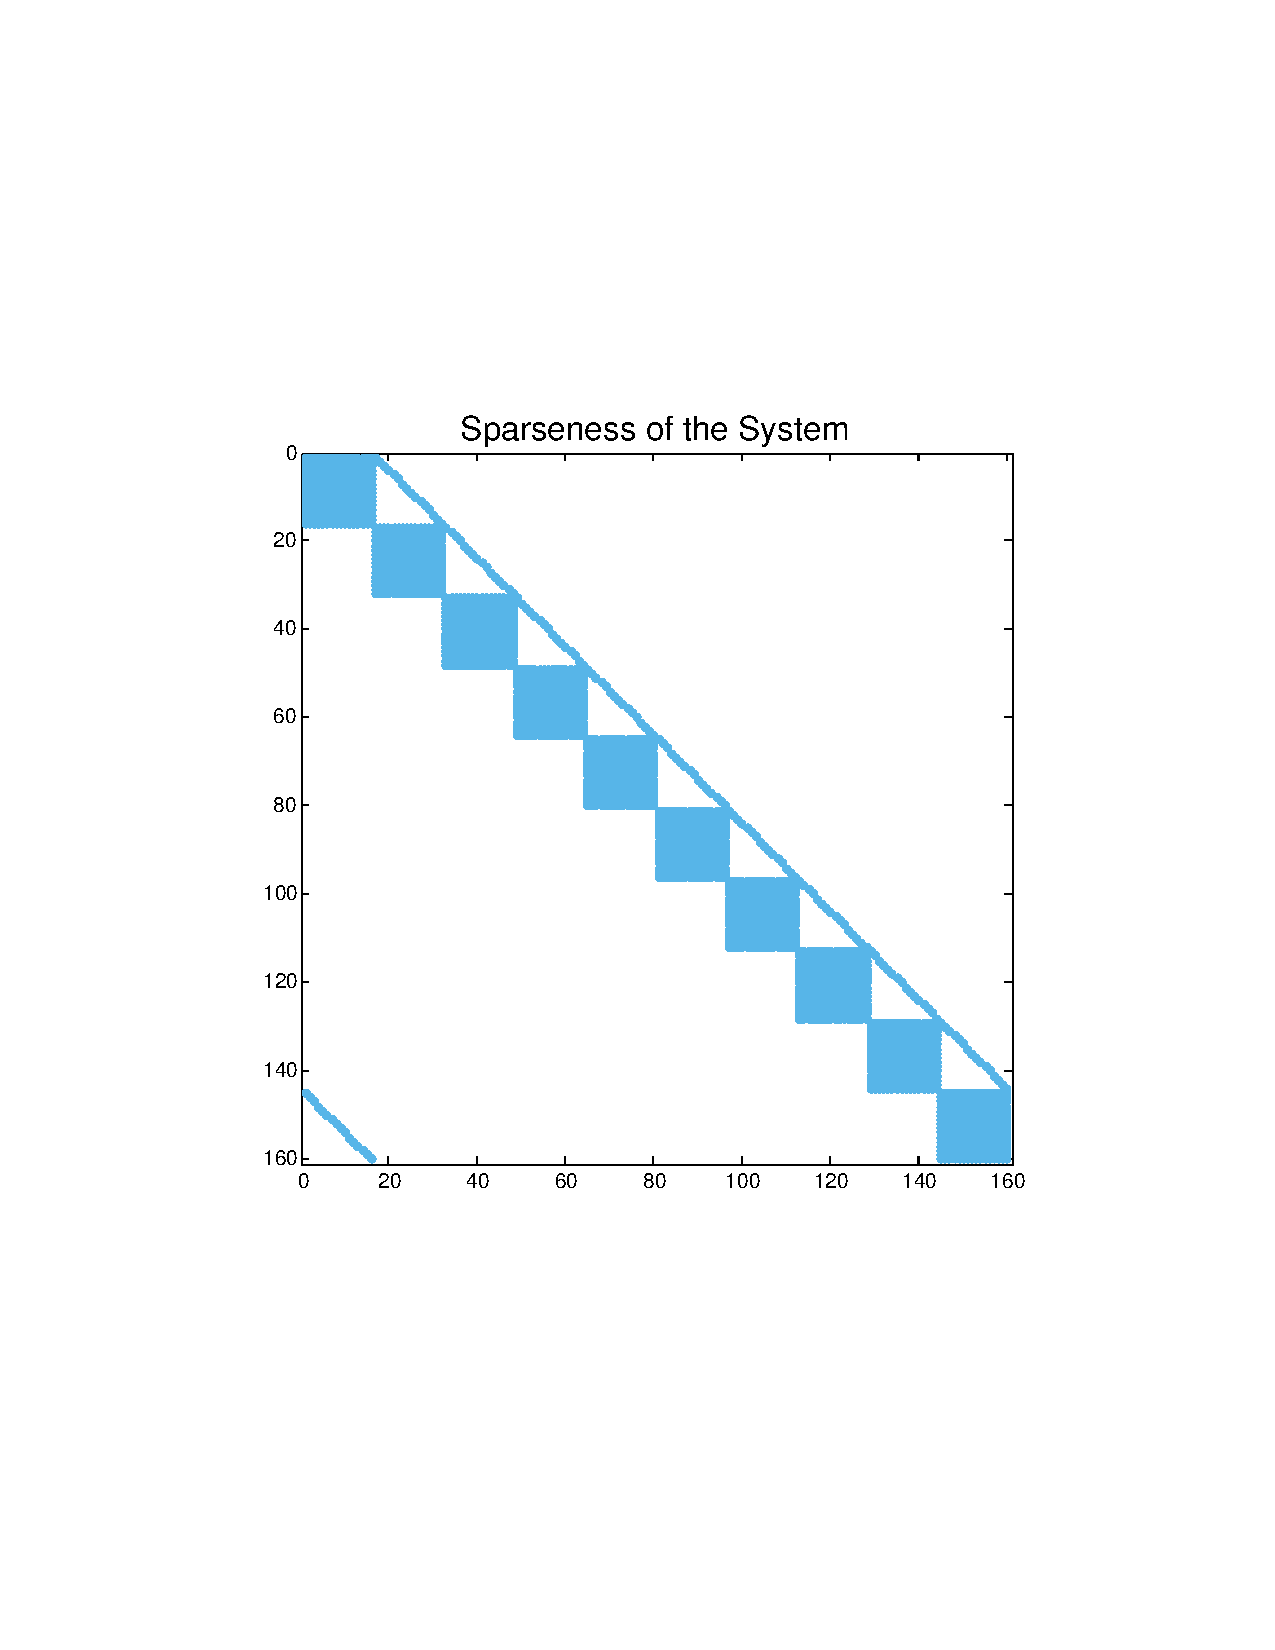
\includegraphics[clip=true, trim=20 30 20 20, width=0.4\linewidth]{assets/sparseness-of-system.pdf}
    \caption{Structure of the system in \equref{eq:system}.}
    \label{fig:sparseness-of-system}
  \end{minipage}
  \hspace{5pt}
  \begin{minipage}{0.45\linewidth}
    \centering
    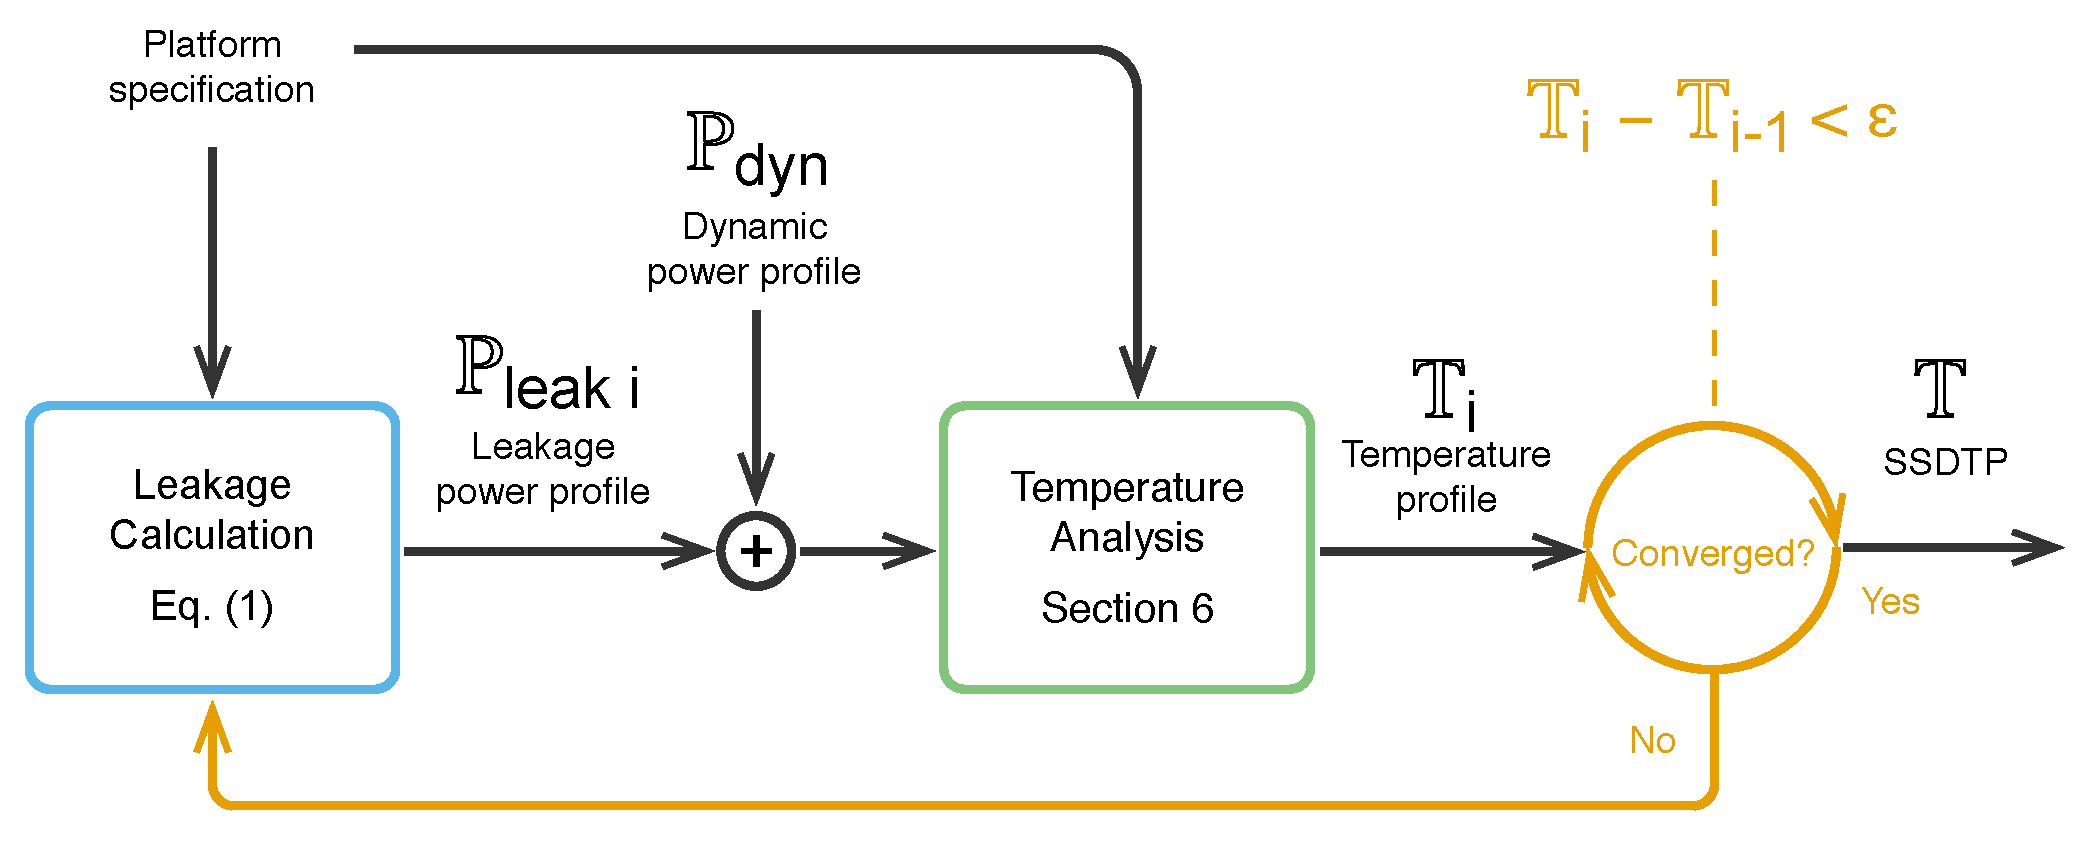
\includegraphics[width=0.9\linewidth]{assets/leakage.pdf}
    \caption{SSDTP with leakage modeling.}
    \label{fig:leakage}
  \end{minipage}
\end{figure*}

Let us start with the discussion on the above-mentioned specific structure of the matrix in \equref{eq:system} and depicted in \figref{fig:sparseness-of-system}. It can be seen that non-zero elements, marked with blue points in the figure, are located only on the block diagonal, one subdiagonal just above the block diagonal, and one subdiagonal in the left bottom corner. The block diagonal is composed of $N_n \times N_n$ matrices while all elements of the subdiagonals are equal to $-1$. Linear systems with the same structure arise in boundary value problems for ODEs where a technique to solve them is to form a so-called condensed equation (CE), or condensed system \cite{stoer2002}.

\isubsection{Auxiliary Transformation} \label{sec:ce-auxiliary}
The analytical solution in \equref{eq:solution} includes two computationally expensive operations, namely the matrix exponential and inverse involving \mbox{$\m{A} = - \m{C}^{-1} \: \m{G}$}, which is an arbitrary square matrix. It is preferable to have a symmetric matrix to perform these computations, since for a real symmetric matrix $\m{M}$ the following eigenvalue decomposition with independent eigenvectors holds \cite{press2007}:
\begin{equation} \label{eq:eigenvalue-decomposition}
  \m{M} = \m{U} \m{\Lambda} \m{U}^\v{T}
\end{equation}
where $\m{U}$ is a square matrix of the eigenvectors, $\m{U}^T$ is the transpose of $\m{U}$, and $\m{\Lambda}$ is a diagonal matrix of the eigenvalues $\lambda_i$ of $\m{M}$. With such a decomposition, the calculation of the matrix exponential and inverse becomes trivial: $e^\m{M} = \m{U} \: e^{\m{\Lambda}} \: \m{U}^\v{T}$ and $\m{M}^{-1} = \m{U} \: \m{\Lambda}^{-1} \: \m{U}^\v{T}$, where the central matrices are diagonal with elements $e^{\lambda_i}$ and $\lambda_i^{-1}$, respectively.

The conductance matrix $\m{G}$ is a symmetric matrix, since if a node A is connected to B, then B is also connected to A with the same conductance \cite{huang2003}. However, as it is mentioned previously, the product of $\m{G}$ with the inverse of the capacitance matrix $\m{C}$ does not have this property. Since $\m{C}$ is a diagonal matrix, we use the following transformation in order to keep the desired symmetry:
\begin{equation} \label{eq:substitution}
  \tilde{\v{T}}(t) = \m{C}^{\frac{1}{2}} \v{T}(t) \hs \tilde{\m{A}} = -\m{C}^{-\frac{1}{2}} \m{G} \: \m{C}^{-\frac{1}{2}}
\end{equation}
where $\tm{A}$ is symmetric, since $\tm{A}^T = -(\m{C}^{-\half} \m{G} \m{C}^{-\half})^T = -(\m{C}^{-\half})^T \m{G}^T (\m{C}^{-\half})^T = \tilde{\m{A}}$. Consequently, the system of ODEs (\equref{eq:fourier-model}) and its solutions (\equref{eq:solution}) can be rewritten as the following:
\begin{align*}
  & \frac{d\tilde{\v{T}}(t)}{dt} = \tilde{\m{A}} \: \m{Y}(t) + \m{C}^{-\frac{1}{2}} \v{P} \\
  & \tilde{\v{T}}(t) = e^{\tilde{\m{A}} t} \tilde{\v{T}}_0 + \tilde{\m{A}}^{-1} (e^{\tilde{\m{A}} t} - \m{I}) \m{C}^{-\frac{1}{2}} \v{P}
\end{align*}
where $\tilde{\m{A}}$ is a symmetric matrix. Therefore, in the case of, e.g., the matrix exponential we have:
\begin{equation} \label{eq:matrix-exponential}
  e^{\tm{A} t} = \m{U} \: e^{\m{\Lambda} t} \: \m{U}^T = \m{U} \: \diag{e^{t \lambda_0}}{e^{t \lambda_{N_n - 1}}} \: \m{U}^T
\end{equation}
where $diag$ denotes a diagonal matrix and $\lambda_i$ are the eigenvalues of $\tm{A}$. A similar equation can be obtained for $\tm{A}^{-1}$.

The next step is to update the SSDTP system in \equref{eq:recurrent-system}:
\begin{align}
  & \tv{T}_{i+1} = \tm{K}_i \: \tv{T}_i + \tm{B}_i \: \v{P}_i \label{eq:recurrent-equation} \\
  & \tm{K}_i = e^{\tm{A} \: \Delta t_i} \hs \tm{B}_i = \tm{A}^{-1} \left( e^{\tm{A} \Delta t_i} - \m{I} \right) \m{C}^{-\frac{1}{2}} \nonumber
\end{align}
Using the eigenvalue decomposition, the last equation can be computed in the following way:
\[
  \tm{B}_i = \m{U} \: \diag{\frac{e^{\Delta t_i \: \lambda_0} - 1}{\lambda_0}}{\frac{e^{\Delta t_i \: \lambda_{N_n - 1}} - 1}{\lambda_{N_n - 1}}} \: \m{U}^T \: \m{C}^{-\frac{1}{2}}
\]

\isubsection{Solution with Condensed Equation (CE)} \label{sec:ce-solution}
Let us return back to the recurrent system given by \equref{eq:recurrent-equation} and denote \mbox{$\m{Q}_i = \tm{B}_i \: \v{P}_i$}:
\begin{align}
  & \tv{T}_{i + 1} = \tm{K}_i \: \tv{T}_i + \m{Q}_i, \; i = \range{0}{N_s - 1} \label{eq:ce-recurrent} \\
  & \tv{T}_0 = \tv{T}_{N_s + 1} \nonumber
\end{align}
In order to form the condensed equation mentioned in the beginning of this section, we perform the iterative repetition of \equref{eq:ce-recurrent} that leads to:
\begin{equation} \label{eq:y-recurrent}
  \tv{T}_i = \prod_{j = 0}^{i - 1} \tm{K}_j \: \tv{T}_0 + \m{W}_{i - 1}, \; i = \range{1}{N_s}
\end{equation}
where $\m{W}_i$ are defined as the following:
\begin{equation}
  \m{W}_0 = \m{Q}_0 \hspace{15pt} \m{W}_i = \tm{K}_i \: \m{W}_{i - 1} + \m{Q}_i, \; i = \range{1}{N_s - 1} \label{eq:p-recurrent}
  % \m{W}_i & = \sum_{l = 1}^i \prod_{j = l}^i \tilde{\m{K}}_j \: \m{Q}_{l - 1} + \m{Q}_i, \: i = \range{1}{N_s - 1} \nonumber \\
\end{equation}
We calculate the final vector $\tilde{\v{T}}_{N_s}$ using \equref{eq:y-recurrent} and \equref{eq:p-recurrent}:
\[
  \tilde{\v{T}}_{N_s} = \prod_{j = 0}^{N_s - 1} \tilde{\m{K}}_j \: \tilde{\v{T}}_0 + \m{W}_{N_s - 1}
\]
Taking into account the boundary condition given by \equref{eq:boundary-condition}, we obtain the following system of linear equations:
\begin{equation} \label{eq:core-system}
  (\m{I} - \prod_{j = 0}^{N_s - 1} \tm{K}_j) \: \tv{T}_0 = \m{W}_{N_s - 1}
\end{equation}
We recall that $\tm{K}_i$ is the matrix exponential given by \equref{eq:matrix-exponential}, therefore, the following simplification holds:
% \[
%   \prod_{j = i}^l \tm{K}_j = \prod_{j = i}^l e^{\tm{A} \Delta t_j} = e^{\tm{A} \sum_{j = i}^l \Delta t_j} = \m{U} e^{\left( \sum_{j = i}^l \Delta t_j \: \m{\Lambda} \right)} \m{U}^T
% \]
% Consequently:
\[
  \prod_{j = 0}^{N_s - 1} \tm{K}_j = \m{U} \: \diag{e^{\period \lambda_0}}{e^{\period \lambda_{N_n - 1}}} \: \m{U}^T
\]
where $\period$ is the application period. Substituting this product into \equref{eq:core-system}, we obtain the following system:
\[
  (\m{I} - \m{U} \: e^{\period \m{\Lambda}} \: \m{U}^T) \: \tv{T}_0 = \m{W}_{N_s - 1}
\]
The identity matrix $\m{I}$ can be split into $\m{U} \m{U}^T$, hence:
\begin{equation} \label{eq:t0}
  \tv{T}_0 = \m{U} \: (\m{I} - e^{\period \m{\Lambda}})^{-1} \: \m{U}^T \: \m{W}_{N_s - 1} = \m{Z} \: \m{W}_{N_s - 1}
\end{equation}
where:
\[
  \m{Z} = \m{U} \: \diag{\frac{1}{1 - e^{\period \lambda_0}}}{\frac{1}{1 - e^{\period \lambda_{N_n - 1}}}} \: \m{U}^T
\]
The equation gives the initial solution vector $\tv{T}_0$; the rest of the vectors $\tv{T}_i$ are successively found from \equref{eq:ce-recurrent}.
% The equation gives the initial solution vector $\tv{T}_0$, the rest of vectors $\tv{T}_i$ for $i = \range{1}{N_s - 1}$ are successively found from \equref{eq:ce-recurrent}.

Since the power profile is evenly sampled with the sampling interval $\Delta t$, the recurrence in \equref{eq:ce-recurrent} turns into:
\[
  \tv{T}_{i+1} = \tm{K} \: \tv{T}_i + \m{Q}_i = \tm{K} \: \tv{T}_i + \tm{B} \: \v{P}_i
\]
where $\tm{K} = e^{\tm{A} \: \Delta t}$ and $\tm{B} = \tm{A}^{-1} ( e^{\tm{A} \: \Delta t} - \m{I} ) \m{C}^{-\frac{1}{2}}$. Here $\tm{K}$ and $\tm{B}$ are constants, since they depend only on the matrices $\tm{A}$, $\m{C}$, and sampling interval $\Delta t$, which is fixed. In this case, the block diagonal of the matrix $\tilde{\mathbb{A}}$, similar to \equref{eq:system}, is composed of the same repeating block $\tm{K}$ and the recurrent expressions take the following form:
\begin{align}
  & \m{W}_i = \tm{K} \: \m{W}_{i - 1} + \m{Q}_i, \; i = \range{1}{N_s - 1} \label{eq:final-p-recurrence} \\
  & \tv{T}_{i + 1} = \tm{K} \: \tv{T}_i + \m{Q}_i, \; i = \range{0}{N_s - 1} \label{eq:final-y-recurrence}
\end{align}
where $\m{Q}_i = \tm{B} \: \v{P}_i$, $\m{W}_0 = \m{Q}_0$, and $\tv{T}_0$ is given by \equref{eq:t0}.

The last step of the solution is to return to temperature by performing the backward substitution opposite to \equref{eq:substitution}:
\[
  \v{T}_i = \m{C}^{-\frac{1}{2}} \: \tv{T}_i, \: i = \range{0}{N_s - 1}
\]

As we see, the auxiliary substitution from \secref{sec:ce-auxiliary} allows us to perform the single-time eigenvalue decomposition with orthogonal eigenvectors (\equref{eq:eigenvalue-decomposition}) that later eases the computational process at several stages. In \secref{sec:ce-solution} it can be observed that the solution of the system in \equref{eq:system} has been reduced to two successive recurrences in \equref{eq:final-p-recurrence} and \equref{eq:final-y-recurrence} over $N_s$ steps in the power profile, which implies a linear complexity on $N_s$.

It should be mentioned that the eigenvalue decomposition along with $\tm{K}$ and $\tm{B}$ are computed only once for a particular RC thermal circuit and can be considered as a given together with the RC circuit. It has not to be recalculated when a SSDTP is generated, which significantly decreases the computational time.
